%!TEX root = main.tex
\section{Hypothesis Formation and the cycle of visual analysis\label{sec:hypothesis}}
\subsection{Visual Querying in the \textit{Sensemaking Framework}}
In developing \zv, we collaborated with scientists from astronomy, genetics, and material science in a year-long participatory design process~\cite{Lee2017}. In particular, we study how various features impacts analyst's ability to rapidly generate new hypothesis and insights and perform visual querying and analysis. In addition, we were interested in how a visual query system (VQS) like \zv fits into the participant's analysis workflow. Our findings offered design guidelines for improving the usability and adoption of next-generation VQSs. More importantly, in this paper, we focus on applying our findings on visual querying to the context of supporting the full cycle of visual data exploration. We highlight two of the key findings related to this goal below: 

Our participatory design findings points towards future ----- in supporting a cycle of ---.  ----advocate ---cycle of visual analysis. 
\begin{itemize}
	\item Essential ingredient in facilitating intelligent vague querying and exploration.
	\item This is a human process (\cite{Heer2012,Pirolli})
	\item Iterative Hypothesis Exploration/Refinement : argue that the following properties is important to sustain this “cycle of visual analysis” 
\end{itemize}


\stitle{Supporting Complex Vague Expressive Querying}
\zv is an example of a \emph{precise visual querying system (PVQS)}, which accepts precise queries as an input, expressed through interactions or directly specified via ZQL. The expressiveness of PVQSs comes from the multiplicative effect of ------ combinations ---- into a custom workflow, combinations --- workflow. For example, in our participatory design study, we found that ---- (for example, filter first, then examine representative trends, then query with pattern, then adjust filter to update hypothesis, higher lower value). 

The extensibility of these systems or querying language also comes with the cost of potentially overloading the users with too many potential options to chose from. 

\par When users are querying with our VQS (which we now refer to as `precise querying'), they often need to translate their ambiguous, high-level questions into an plan that consists of several interactions in series which addresses the desired query incrementally. However, the combination workflow is limited and sometimes, queries can not be expressed in this framework. Complex multistep queries. Give one example. 
\par despite extensive work in database usability, there is an inevitable design trade-off between the query expressivity and interface usability\cite{Morton2014,Jagadish2007}. In Section~\ref{sec:vague}, we survey related work in this area and advocate for -----. 


Precise querying 

Construction of multi-step queries
- tie in many different types of interactions
- goal is data understanding 

\par Our \zv work ------- Bottom up and top down querying in VQS facilitates rapid insight discovery. 
workflow integration , complex queries,
While our visual interface ---, ----it was unable to capture all the -----. [Give some example queries that didn't work]. Balance between language/querying complexity versus expressiveness. More importantly pointed towards a need for vague querying. Give some examples of vague querying.

\stitle{Top-down and Bottom-up Querying Modalities}
We employed Pirolli and Card's~\cite{Pirolli} information foraging framework for domain-experts to contextualize our study results. Pirolli and Card's notional model distinguishes between information processing tasks that are \textit{top-down} (from theory to data) and \textit{bottom-up} (from data to theory). In the context of visual querying, users employ top-down approaches by starting with a hypothesis on what patterns to look for and express it through sketching or inputting an equation (Figure~\ref{fig:modalities}b,d). On the other hand, bottom-up approaches originate from the data (or equivalently, the visualization). For example, the user may drag and drop a visualization of interest in the dataset as the input query or upload a visualization from an external dataset (Figure~\ref{fig:modalities}a,c). 
\par Our interactions with the scientists showed that \emph{bottom-up querying via drag-and-drop was more intuitive and more commonly used than top-down querying methods when the users have no desired patterns in mind}, which is commonly the case for exploratory data analysis. One of the main reason why participants did not find sketching useful was that they often do not start their analysis with a pattern in mind. Later, their intuition about what to query is derived from other visualizations that they see in the VQS, in which case it made more sense to query using those visualizations as examples directly. Similarly, while functional fitting is a common operation in scientific data analysis, querying by equation is also unpopular, since it is challenging to formulate functional forms in an prescriptive, ad-hoc manner without seeing what the common patterns in the dataset are. 
\par While the usage of each querying feature may vary from one participant to the next, a key design principle that came from this finding was the need for visual query systems to provide visualization recommendations that can help analysts jumpstart their exploration. We found that many users made use of the representative trends and outliers visualizations provided by \zv as contextual information to better understand their data (e.g. after a filter is applied) or to query based on these recommended visualizations (e.g. find visualizations that are similar to the one in the largest representative clusters). 
\par Recommendation facillitate smoother flow of analysis, ensures that user is never stuck or out of ideas. it does this by going towards better data understanding, accurate understanding of the context of analysis and scope of data. should not only close the loop between the two modalities of querying and exploration, but also contribute towards ---- data understanding. In Section~\ref{sec:understanding}, we advocate the importance of building recommenders that contributes towards data understanding but also -----. 


\begin{figure}[h!]
	\label{fig:cycle}
	\centering
	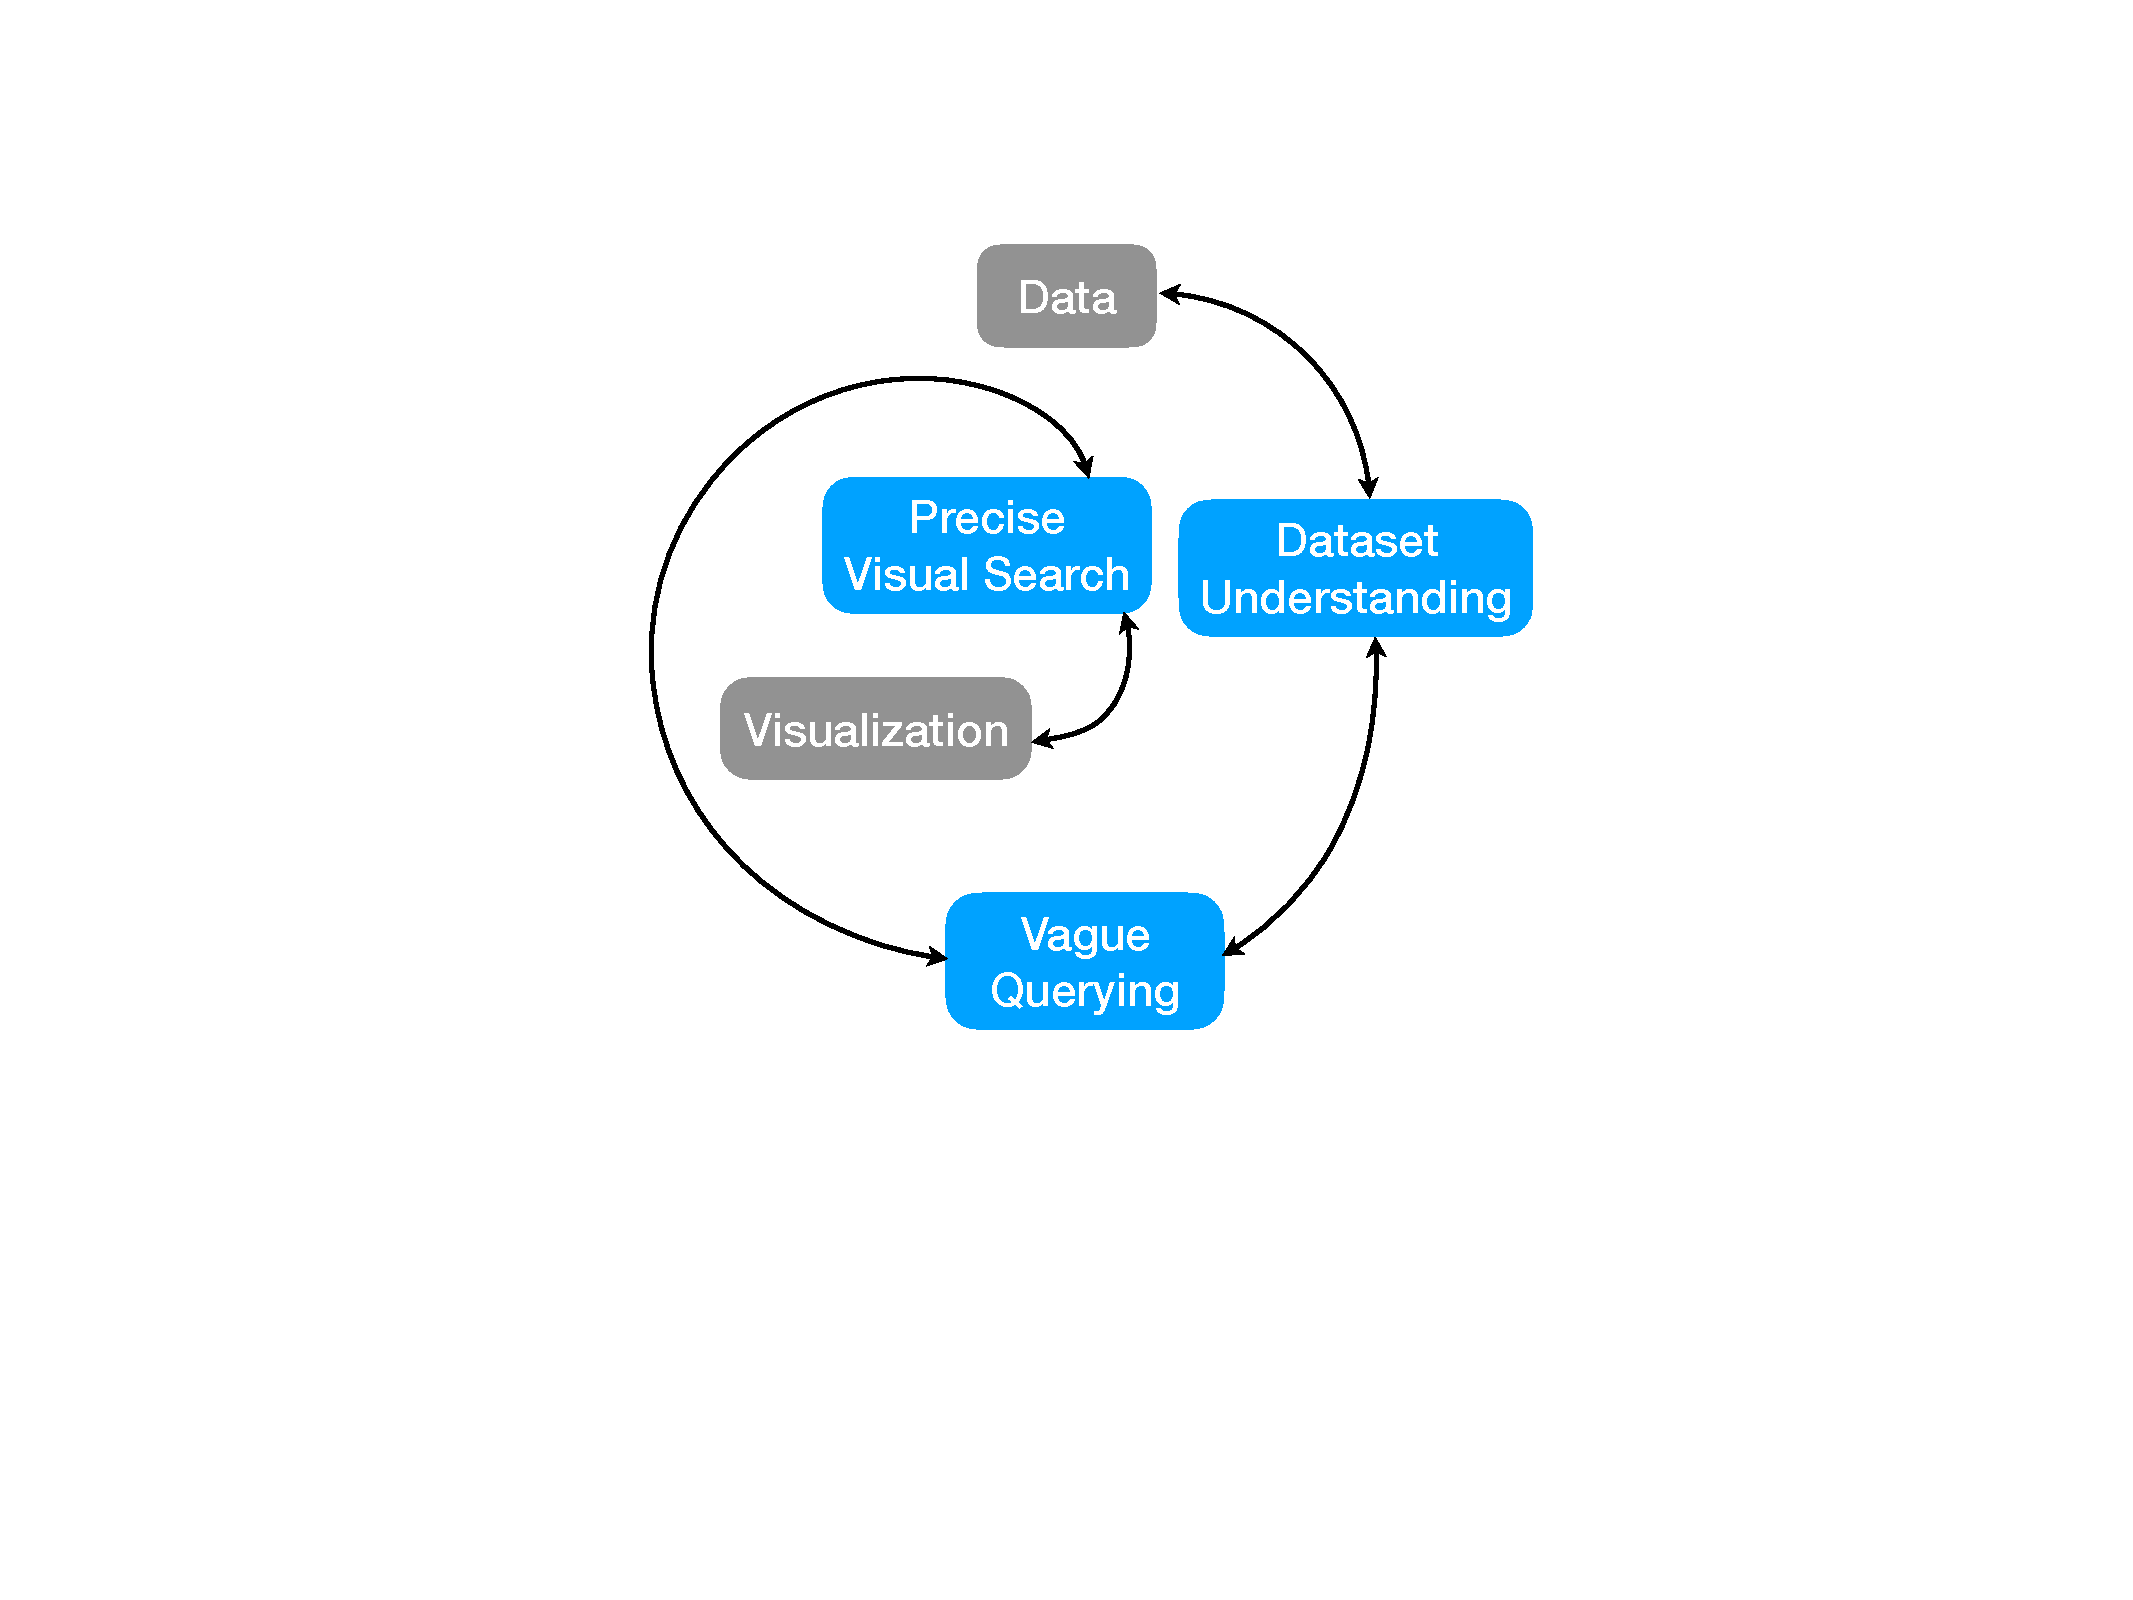
\includegraphics[width=0.5\linewidth]{figures/cycle.pdf}
	\caption{Cycle of visual data exploration.}
\end{figure}

\subsection{Challenges Ahead}
The goal here is to help novice submit precise queries without SQL background, easy to use interface. Our study found that VQS does more than just this, but still not enough.
\begin{itemize}
	\item Precise Search Fail to understand intricacies of user need/intent, need more expressivity/flexibility for querying.
	\item  No perfect training workload, real-world data + task is noisy and complex. 
	\item towards more holistic model for insight discovery
\end{itemize}
